\section{Ejercicios}

\subsection{Nivel básico}

\begin{ejercicio}

Una superficie plana de área \(\SI{0.200}{\metre\squared}\) se encuentra en un
campo eléctrico uniforme de magnitud

\[
E=\SI{500}{\newton\per\coulomb}.
\]

La normal a la superficie forma un ángulo de \(60^\circ\) con el campo.

Determine el flujo eléctrico a través de la superficie.

\end{ejercicio}

\begin{respuesta}

\[
\boxed{\Phi_E=\SI{50.0}{\newton\metre\squared\per\coulomb}}
\]

\end{respuesta}

\begin{explicacion}

Para una superficie plana en un campo uniforme,

\[
\Phi_E=EA\cos\theta,
\]

donde \(\theta\) es el ángulo entre el campo y la normal a la superficie.

Sustituyendo,

\[
\Phi_E=(500)(0.200)\cos60^\circ.
\]

Como

\[
\cos60^\circ=0.500,
\]

resulta

\[
\Phi_E=(500)(0.200)(0.500).
\]

Por tanto,

\[
\boxed{\Phi_E=\SI{50.0}{\newton\metre\squared\per\coulomb}}.
\]

\end{explicacion}


\begin{ejercicio}

Una superficie plana de área \(\SI{0.150}{\metre\squared}\) está sometida a un
campo eléctrico uniforme de magnitud

\[
E=\SI{800}{\newton\per\coulomb}.
\]

El campo forma un ángulo de \(30^\circ\) con el plano de la superficie.

Determine el flujo eléctrico.

\end{ejercicio}

\begin{respuesta}

\[
\boxed{\Phi_E=\SI{60.0}{\newton\metre\squared\per\coulomb}}
\]

\end{respuesta}

\begin{explicacion}

El ángulo de la expresión

\[
\Phi_E=EA\cos\theta
\]

debe medirse respecto de la normal a la superficie.

Como el campo forma \(30^\circ\) con el plano,

\[
\theta=90^\circ-30^\circ=60^\circ.
\]

Entonces,

\[
\Phi_E=(800)(0.150)\cos60^\circ.
\]

Así,

\[
\Phi_E=(800)(0.150)(0.500)
=\SI{60.0}{\newton\metre\squared\per\coulomb}.
\]

Por tanto,

\[
\boxed{\Phi_E=\SI{60.0}{\newton\metre\squared\per\coulomb}}.
\]

\end{explicacion}


\begin{ejercicio}

Una superficie plana de área \(\SI{0.0400}{\metre\squared}\) está en un campo
uniforme de magnitud

\[
E=\SI{1.20e3}{\newton\per\coulomb}.
\]

El campo apunta en sentido opuesto a la normal elegida para la superficie.

Determine el flujo eléctrico.

\end{ejercicio}

\begin{respuesta}

\[
\boxed{\Phi_E=-\SI{48.0}{\newton\metre\squared\per\coulomb}}
\]

\end{respuesta}

\begin{explicacion}

Como el campo y la normal tienen sentidos opuestos,

\[
\theta=180^\circ.
\]

Aplicamos

\[
\Phi_E=EA\cos\theta.
\]

Entonces,

\[
\Phi_E=(1.20\times10^3)(0.0400)\cos180^\circ.
\]

Como

\[
\cos180^\circ=-1,
\]

obtenemos

\[
\boxed{\Phi_E=-\SI{48.0}{\newton\metre\squared\per\coulomb}}.
\]

El signo negativo indica que el campo atraviesa la superficie en sentido contrario
a la normal elegida.

\end{explicacion}


\begin{ejercicio}

Un campo eléctrico uniforme de magnitud

\[
E=\SI{2.00e3}{\newton\per\coulomb}
\]

es paralelo a una superficie plana de área \(\SI{0.500}{\metre\squared}\).

Determine el flujo eléctrico a través de la superficie.

\end{ejercicio}

\begin{respuesta}

\[
\boxed{\Phi_E=0}
\]

\end{respuesta}

\begin{explicacion}

Si el campo es paralelo al plano, forma un ángulo de \(90^\circ\) con la normal.

Entonces,

\[
\Phi_E=EA\cos90^\circ.
\]

Como

\[
\cos90^\circ=0,
\]

resulta

\[
\boxed{\Phi_E=0}.
\]

El campo puede ser distinto de cero aunque el flujo a través de la superficie sea
nulo.

\end{explicacion}


\begin{ejercicio}

Una superficie cerrada encierra las cargas

\[
q_1=+\SI{4.0}{\micro\coulomb},\qquad
q_2=-\SI{1.0}{\micro\coulomb},\qquad
q_3=+\SI{2.0}{\micro\coulomb}.
\]

Determine el flujo eléctrico neto a través de la superficie.

\end{ejercicio}

\begin{respuesta}

\[
\boxed{
\Phi_E\approx+\SI{5.6e5}{\newton\metre\squared\per\coulomb}
}
\]

\end{respuesta}

\begin{explicacion}

Primero calculamos la carga neta encerrada:

\[
Q_{\text{enc}}=q_1+q_2+q_3.
\]

Entonces,

\[
Q_{\text{enc}}=(4.0-1.0+2.0)\,\si{\micro\coulomb}
=\SI{5.0}{\micro\coulomb}.
\]

Aplicamos la ley de Gauss:

\[
\Phi_E=\frac{Q_{\text{enc}}}{\varepsilon_0}.
\]

Sustituyendo,

\[
\Phi_E=
\frac{5.0\times10^{-6}}{8.854\times10^{-12}}
\approx
\SI{5.6e5}{\newton\metre\squared\per\coulomb}.
\]

Por tanto,

\[
\boxed{
\Phi_E\approx+\SI{5.6e5}{\newton\metre\squared\per\coulomb}
}.
\]

El signo positivo indica un flujo neto saliente.

\end{explicacion}


\begin{ejercicio}

El flujo eléctrico neto a través de una superficie cerrada es

\[
\Phi_E=-\SI{3.39e5}{\newton\metre\squared\per\coulomb}.
\]

Determine la carga neta encerrada.

\end{ejercicio}

\begin{respuesta}

\[
\boxed{Q_{\text{enc}}\approx-\SI{3.00}{\micro\coulomb}}
\]

\end{respuesta}

\begin{explicacion}

La ley de Gauss establece

\[
\Phi_E=\frac{Q_{\text{enc}}}{\varepsilon_0}.
\]

Despejamos:

\[
Q_{\text{enc}}=\varepsilon_0\Phi_E.
\]

Sustituyendo,

\[
Q_{\text{enc}}
=(8.854\times10^{-12})(-3.39\times10^5)
\approx-3.00\times10^{-6}\,\si{\coulomb}.
\]

Por tanto,

\[
\boxed{Q_{\text{enc}}\approx-\SI{3.00}{\micro\coulomb}}.
\]

El signo negativo indica que la carga neta encerrada es negativa.

\end{explicacion}


\begin{ejercicio}

Una carga puntual positiva se encuentra fuera de una superficie cerrada. No existe
ninguna carga dentro de la superficie.

¿Puede existir campo eléctrico sobre la superficie? ¿Cuál es el flujo eléctrico neto?

\end{ejercicio}

\begin{respuesta}

Sí, puede existir campo eléctrico sobre la superficie.

\[
\boxed{\Phi_E=0}
\]

\end{respuesta}

\begin{explicacion}

La carga externa produce un campo eléctrico que puede ser distinto de cero sobre
todos los puntos de la superficie.

Sin embargo, la superficie no encierra carga:

\[
Q_{\text{enc}}=0.
\]

Por la ley de Gauss,

\[
\Phi_E=\frac{Q_{\text{enc}}}{\varepsilon_0}=0.
\]

Por tanto,

\[
\boxed{\Phi_E=0}.
\]

Las contribuciones del campo que entra en la superficie se compensan con las que
salen.

\end{explicacion}


\begin{ejercicio}

Una carga puntual \(+q\) se encuentra dentro de una superficie cerrada.

Indique qué sucede con el flujo eléctrico neto si:

\begin{enumerate}
    \item se duplica el tamaño de la superficie sin que la carga salga;
    \item la superficie cambia de una esfera a un cubo;
    \item la carga se desplaza a otro punto del interior.
\end{enumerate}

\end{ejercicio}

\begin{respuesta}

En los tres casos el flujo permanece igual:

\[
\boxed{\Phi_E=\frac{q}{\varepsilon_0}}
\]

\end{respuesta}

\begin{explicacion}

La ley de Gauss establece

\[
\Phi_E=\frac{Q_{\text{enc}}}{\varepsilon_0}.
\]

En las tres modificaciones la carga encerrada continúa siendo

\[
Q_{\text{enc}}=q.
\]

Por ello, ni el tamaño, ni la forma de la superficie, ni la posición de la carga
dentro de ella modifican el flujo neto.

Así,

\[
\boxed{\Phi_E=\frac{q}{\varepsilon_0}}.
\]

La distribución local del campo sobre la superficie sí puede cambiar.

\end{explicacion}


\begin{ejercicio}

Un cubo de lado

\[
L=\SI{0.200}{\metre}
\]

se encuentra en un campo eléctrico uniforme de magnitud

\[
E=\SI{3.00e2}{\newton\per\coulomb}
\]

dirigido horizontalmente hacia la derecha.

\begin{center}
\begin{tikzpicture}[>=Latex,scale=0.85]

\draw[thick] (0,0) rectangle (4,4);

\foreach \y in {0.5,1.5,2.5,3.5}
    \draw[->,thick] (-1,\y) -- (5,\y);

\node at (5.45,3.5) {$E$};
\node[left] at (0,2) {$S_L$};
\node[right] at (4,2) {$S_R$};
\node[below] at (2,0) {$L$};

\end{tikzpicture}
\end{center}

Determine el flujo a través de la cara izquierda, la cara derecha y el flujo neto
a través del cubo.

\end{ejercicio}

\begin{respuesta}

\[
\boxed{
\Phi_L=-\SI{12.0}{\newton\metre\squared\per\coulomb}
}
\]

\[
\boxed{
\Phi_R=+\SI{12.0}{\newton\metre\squared\per\coulomb}
}
\]

\[
\boxed{\Phi_{\text{neto}}=0}
\]

\end{respuesta}

\begin{explicacion}

El área de cada cara es

\[
A=L^2=(0.200)^2=\SI{0.0400}{\metre\squared}.
\]

En la cara derecha, el campo tiene el mismo sentido que la normal exterior:

\[
\Phi_R=EA.
\]

Entonces,

\[
\Phi_R=(300)(0.0400)
=\SI{12.0}{\newton\metre\squared\per\coulomb}.
\]

Por tanto,

\[
\boxed{
\Phi_R=+\SI{12.0}{\newton\metre\squared\per\coulomb}
}.
\]

En la cara izquierda, el campo es opuesto a la normal exterior:

\[
\Phi_L=-EA,
\]

de modo que

\[
\boxed{
\Phi_L=-\SI{12.0}{\newton\metre\squared\per\coulomb}
}.
\]

En las otras cuatro caras el campo es paralelo a las superficies y, por tanto,

\[
\Phi=0.
\]

El flujo neto es

\[
\Phi_{\text{neto}}
=\Phi_L+\Phi_R
=-12.0+12.0=0.
\]

Así,

\[
\boxed{\Phi_{\text{neto}}=0}.
\]

\end{explicacion}


\begin{ejercicio}

Indique la superficie gaussiana más conveniente para calcular el campo eléctrico
en cada distribución ideal:

\begin{enumerate}
    \item una carga puntual;
    \item una línea recta infinita uniformemente cargada;
    \item una lámina infinita uniformemente cargada.
\end{enumerate}

\end{ejercicio}

\begin{respuesta}

\begin{enumerate}
    \item Una esfera centrada en la carga.
    \item Un cilindro coaxial con la línea.
    \item Una pastilla cilíndrica que atraviese la lámina.
\end{enumerate}

\end{respuesta}

\begin{explicacion}

La superficie gaussiana debe elegirse de acuerdo con la simetría de la distribución.

Para una carga puntual existe simetría esférica, por lo que conviene una esfera.

Para una línea infinita existe simetría cilíndrica, por lo que conviene un cilindro
coaxial.

Para una lámina infinita existe simetría plana, por lo que una pastilla cilíndrica
permite separar las caras que aportan flujo de la superficie lateral, cuyo flujo es
nulo.

La ley de Gauss es válida para otras superficies, pero estas elecciones permiten
simplificar el cálculo del campo.

\end{explicacion}


\subsection{Nivel intermedio}

\begin{ejercicio}

Una carga puntual

\[
Q=+\SI{6.00}{\micro\coulomb}
\]

se encuentra en el centro de una superficie gaussiana esférica de radio

\[
r=\SI{0.300}{\metre}.
\]

Utilice la ley de Gauss para determinar la magnitud del campo eléctrico sobre la
superficie.

\end{ejercicio}

\begin{respuesta}

\[
\boxed{E\approx\SI{5.99e5}{\newton\per\coulomb}}
\]

El campo apunta radialmente hacia afuera.

\end{respuesta}

\begin{explicacion}

Por simetría esférica, el campo tiene la misma magnitud en todos los puntos de la
superficie y es perpendicular a ella.

Por tanto,

\[
\Phi_E=E(4\pi r^2).
\]

La carga encerrada es

\[
Q_{\text{enc}}=Q.
\]

Aplicamos Gauss:

\[
E(4\pi r^2)=\frac{Q}{\varepsilon_0}.
\]

Despejando,

\[
E=\frac{Q}{4\pi\varepsilon_0r^2}
=k\frac{Q}{r^2}.
\]

Sustituyendo,

\[
E=(8.99\times10^9)
\frac{6.00\times10^{-6}}{(0.300)^2}.
\]

Entonces,

\[
\boxed{E\approx\SI{5.99e5}{\newton\per\coulomb}}.
\]

Como la carga es positiva, el campo apunta radialmente hacia afuera.

\end{explicacion}


\begin{ejercicio}

Una cáscara esférica delgada no conductora de radio

\[
R=\SI{0.200}{\metre}
\]

posee una carga uniforme total

\[
Q=+\SI{8.00}{\micro\coulomb}.
\]

Determine el campo eléctrico a las distancias:

\[
r_1=\SI{0.100}{\metre},
\qquad
r_2=\SI{0.400}{\metre}.
\]

\end{ejercicio}

\begin{respuesta}

\[
\boxed{E(r_1)=0}
\]

\[
\boxed{E(r_2)\approx\SI{4.49e5}{\newton\per\coulomb}}
\]

\end{respuesta}

\begin{explicacion}

Para

\[
r_1<R,
\]

una superficie gaussiana esférica de radio \(r_1\) no encierra carga:

\[
Q_{\text{enc}}=0.
\]

Entonces,

\[
E(4\pi r_1^2)=0,
\]

por lo que

\[
\boxed{E(r_1)=0}.
\]

Para

\[
r_2>R,
\]

la superficie gaussiana encierra toda la carga:

\[
Q_{\text{enc}}=Q.
\]

Así,

\[
E=k\frac{|Q|}{r_2^2}.
\]

Sustituyendo,

\[
E=(8.99\times10^9)
\frac{8.00\times10^{-6}}{(0.400)^2}.
\]

Por tanto,

\[
\boxed{E(r_2)\approx\SI{4.49e5}{\newton\per\coulomb}}.
\]

\end{explicacion}


\begin{ejercicio}

Una esfera sólida aislante de radio

\[
R=\SI{0.200}{\metre}
\]

contiene una carga total uniforme

\[
Q=+\SI{8.00}{\micro\coulomb}.
\]

Determine la magnitud del campo eléctrico en:

\[
r_1=\SI{0.100}{\metre},\qquad
r_2=\SI{0.200}{\metre},\qquad
r_3=\SI{0.400}{\metre}.
\]

\end{ejercicio}

\begin{respuesta}

\[
\boxed{E(r_1)\approx\SI{8.99e5}{\newton\per\coulomb}}
\]

\[
\boxed{E(r_2)\approx\SI{1.80e6}{\newton\per\coulomb}}
\]

\[
\boxed{E(r_3)\approx\SI{4.49e5}{\newton\per\coulomb}}
\]

\end{respuesta}

\begin{explicacion}

Dentro de una esfera uniformemente cargada,

\[
E=k\frac{|Q|}{R^3}r.
\]

Para \(r_1=\SI{0.100}{\metre}\),

\[
E(r_1)
=(8.99\times10^9)
\frac{(8.00\times10^{-6})(0.100)}{(0.200)^3}.
\]

Entonces,

\[
\boxed{E(r_1)\approx\SI{8.99e5}{\newton\per\coulomb}}.
\]

En la superficie,

\[
E(R)=k\frac{|Q|}{R^2},
\]

por lo que

\[
E(r_2)
=(8.99\times10^9)
\frac{8.00\times10^{-6}}{(0.200)^2}
\approx\SI{1.80e6}{\newton\per\coulomb}.
\]

Así,

\[
\boxed{E(r_2)\approx\SI{1.80e6}{\newton\per\coulomb}}.
\]

Para \(r_3>R\), toda la esfera se comporta exteriormente como una carga puntual:

\[
E(r_3)=k\frac{|Q|}{r_3^2}.
\]

Entonces,

\[
E(r_3)
=(8.99\times10^9)
\frac{8.00\times10^{-6}}{(0.400)^2}
\approx\SI{4.49e5}{\newton\per\coulomb}.
\]

Por tanto,

\[
\boxed{E(r_3)\approx\SI{4.49e5}{\newton\per\coulomb}}.
\]

\end{explicacion}


\begin{ejercicio}

Una línea recta infinita posee una densidad lineal uniforme

\[
\lambda=+\SI{3.00}{\micro\coulomb\per\metre}.
\]

Determine la magnitud del campo eléctrico a una distancia perpendicular

\[
r=\SI{0.100}{\metre}.
\]

\end{ejercicio}

\begin{respuesta}

\[
\boxed{E\approx\SI{5.39e5}{\newton\per\coulomb}}
\]

\end{respuesta}

\begin{explicacion}

Elegimos una superficie gaussiana cilíndrica coaxial con la línea.

El flujo sólo atraviesa la superficie lateral:

\[
\Phi_E=E(2\pi rL).
\]

La carga encerrada es

\[
Q_{\text{enc}}=\lambda L.
\]

Aplicando Gauss,

\[
E(2\pi rL)=\frac{\lambda L}{\varepsilon_0}.
\]

Cancelamos \(L\):

\[
E=\frac{|\lambda|}{2\pi\varepsilon_0r}.
\]

Sustituyendo,

\[
E=
\frac{3.00\times10^{-6}}
{2\pi(8.854\times10^{-12})(0.100)}.
\]

Por tanto,

\[
\boxed{E\approx\SI{5.39e5}{\newton\per\coulomb}}.
\]

Como \(\lambda>0\), el campo apunta alejándose de la línea.

\end{explicacion}


\begin{ejercicio}

El campo eléctrico producido por una línea infinita uniformemente cargada tiene
magnitud \(E_1\) a una distancia \(r\).

¿Cuál es la magnitud del campo a una distancia \(3r\)?

\end{ejercicio}

\begin{respuesta}

\[
\boxed{E_2=\frac{E_1}{3}}
\]

\end{respuesta}

\begin{explicacion}

Para una línea infinita,

\[
E=\frac{|\lambda|}{2\pi\varepsilon_0r}.
\]

Por tanto,

\[
E\propto\frac{1}{r}.
\]

Si

\[
r_2=3r_1,
\]

entonces

\[
\frac{E_2}{E_1}
=
\frac{r_1}{r_2}
=
\frac13.
\]

Así,

\[
\boxed{E_2=\frac{E_1}{3}}.
\]

A diferencia del campo de una carga puntual, aquí la dependencia es \(1/r\), no
\(1/r^2\).

\end{explicacion}


\begin{ejercicio}

Una lámina plana infinita no conductora tiene una densidad superficial uniforme

\[
\sigma=+\SI{4.00}{\micro\coulomb\per\metre\squared}.
\]

Determine la magnitud del campo eléctrico a cada lado de la lámina.

\end{ejercicio}

\begin{respuesta}

\[
\boxed{E\approx\SI{2.26e5}{\newton\per\coulomb}}
\]

en ambos lados, alejándose de la lámina.

\end{respuesta}

\begin{explicacion}

Para una lámina infinita uniformemente cargada,

\[
E=\frac{|\sigma|}{2\varepsilon_0}.
\]

Sustituyendo,

\[
E=
\frac{4.00\times10^{-6}}
{2(8.854\times10^{-12})}.
\]

Entonces,

\[
\boxed{E\approx\SI{2.26e5}{\newton\per\coulomb}}.
\]

La magnitud es la misma a ambos lados y no depende de la distancia.

Como la lámina tiene carga positiva, el campo apunta alejándose de ella.

\end{explicacion}


\begin{ejercicio}

Dos láminas infinitas paralelas están situadas perpendicularmente al eje \(x\).
La lámina izquierda posee densidad

\[
+\sigma=+\SI{3.00}{\micro\coulomb\per\metre\squared}
\]

y la derecha

\[
-\sigma=-\SI{3.00}{\micro\coulomb\per\metre\squared}.
\]

Determine el campo eléctrico:

\begin{enumerate}
    \item a la izquierda de ambas láminas;
    \item entre las láminas;
    \item a la derecha de ambas.
\end{enumerate}

\end{ejercicio}

\begin{respuesta}

Fuera de las láminas,

\[
\boxed{E_x=0}.
\]

Entre ellas,

\[
\boxed{E_x\approx+\SI{3.39e5}{\newton\per\coulomb}},
\]

dirigido desde la lámina positiva hacia la negativa.

\end{respuesta}

\begin{explicacion}

Cada lámina produce un campo de magnitud

\[
E_0=\frac{|\sigma|}{2\varepsilon_0}.
\]

Sustituyendo,

\[
E_0=
\frac{3.00\times10^{-6}}
{2(8.854\times10^{-12})}
\approx\SI{1.69e5}{\newton\per\coulomb}.
\]

A la izquierda de ambas láminas, los dos campos tienen igual magnitud y sentidos
opuestos, por lo que

\[
\boxed{E_x=0}.
\]

Entre las láminas, el campo de la lámina positiva apunta hacia la derecha y el de
la lámina negativa también apunta hacia la derecha.

Entonces,

\[
E_x=E_0+E_0=2E_0.
\]

Por tanto,

\[
\boxed{E_x\approx+\SI{3.39e5}{\newton\per\coulomb}}.
\]

A la derecha de ambas láminas, las contribuciones vuelven a tener igual magnitud y
sentidos opuestos:

\[
\boxed{E_x=0}.
\]

\end{explicacion}


\begin{ejercicio}

Una esfera aislante posee una densidad volumétrica uniforme

\[
\rho=\SI{2.00}{\micro\coulomb\per\metre\cubed}.
\]

Se considera una superficie gaussiana esférica de radio

\[
r=\SI{0.100}{\metre}
\]

completamente contenida dentro de la distribución.

Determine:

\begin{enumerate}
    \item la carga encerrada;
    \item el flujo eléctrico;
    \item la magnitud del campo sobre la superficie gaussiana.
\end{enumerate}

\end{ejercicio}

\begin{respuesta}

\[
\boxed{Q_{\text{enc}}\approx\SI{8.38}{\nano\coulomb}}
\]

\[
\boxed{
\Phi_E\approx
\SI{9.46e2}{\newton\metre\squared\per\coulomb}
}
\]

\[
\boxed{E\approx\SI{7.53e3}{\newton\per\coulomb}}
\]

\end{respuesta}

\begin{explicacion}

La carga encerrada es

\[
Q_{\text{enc}}=\rho V.
\]

El volumen de la esfera gaussiana es

\[
V=\frac43\pi r^3.
\]

Entonces,

\[
Q_{\text{enc}}
=(2.00\times10^{-6})
\frac43\pi(0.100)^3.
\]

Por tanto,

\[
\boxed{Q_{\text{enc}}\approx\SI{8.38}{\nano\coulomb}}.
\]

El flujo se obtiene con Gauss:

\[
\Phi_E=\frac{Q_{\text{enc}}}{\varepsilon_0}.
\]

Así,

\[
\boxed{
\Phi_E\approx
\SI{9.46e2}{\newton\metre\squared\per\coulomb}
}.
\]

Por simetría esférica,

\[
\Phi_E=E(4\pi r^2).
\]

Por tanto,

\[
E=\frac{\Phi_E}{4\pi r^2}.
\]

Sustituyendo,

\[
\boxed{E\approx\SI{7.53e3}{\newton\per\coulomb}}.
\]

\end{explicacion}


\begin{ejercicio}

Una carga puntual

\[
q=+\SI{6.00}{\micro\coulomb}
\]

está exactamente en el centro de un cubo.

Determine:

\begin{enumerate}
    \item el flujo eléctrico neto a través de todo el cubo;
    \item el flujo a través de cada una de sus seis caras.
\end{enumerate}

\end{ejercicio}

\begin{respuesta}

\[
\boxed{
\Phi_{\text{total}}
\approx
\SI{6.78e5}{\newton\metre\squared\per\coulomb}
}
\]

\[
\boxed{
\Phi_{\text{cara}}
\approx
\SI{1.13e5}{\newton\metre\squared\per\coulomb}
}
\]

\end{respuesta}

\begin{explicacion}

La carga encerrada es

\[
Q_{\text{enc}}=q.
\]

Por la ley de Gauss,

\[
\Phi_{\text{total}}=\frac{q}{\varepsilon_0}.
\]

Entonces,

\[
\Phi_{\text{total}}
=
\frac{6.00\times10^{-6}}{8.854\times10^{-12}}
\approx
\SI{6.78e5}{\newton\metre\squared\per\coulomb}.
\]

Así,

\[
\boxed{
\Phi_{\text{total}}
\approx
\SI{6.78e5}{\newton\metre\squared\per\coulomb}
}.
\]

Como la carga está en el centro, la simetría del cubo hace que las seis caras reciban
la misma fracción del flujo:

\[
\Phi_{\text{cara}}
=
\frac{\Phi_{\text{total}}}{6}.
\]

Por tanto,

\[
\boxed{
\Phi_{\text{cara}}
\approx
\SI{1.13e5}{\newton\metre\squared\per\coulomb}
}.
\]

\end{explicacion}


\begin{ejercicio}

La figura muestra una superficie gaussiana cerrada. Las cargas \(q_1\) y \(q_2\)
están dentro de ella y \(q_3\) está fuera.

\[
q_1=+\SI{4.00}{\micro\coulomb},\qquad
q_2=-\SI{1.00}{\micro\coulomb},\qquad
q_3=+\SI{5.00}{\micro\coulomb}.
\]

\begin{center}
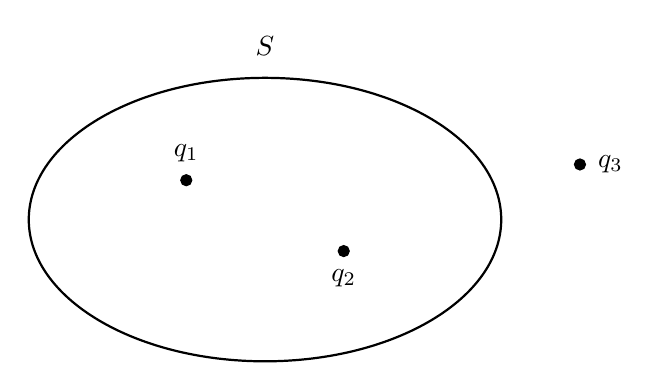
\begin{tikzpicture}[scale=1]

\draw[thick] (0,0) ellipse (3 and 1.8);

\filldraw (-1,0.5) circle (2pt)
node[above=3pt] {$q_1$};

\filldraw (1,-0.4) circle (2pt)
node[below=3pt] {$q_2$};

\filldraw (4,0.7) circle (2pt)
node[right=3pt] {$q_3$};

\node at (0,2.2) {$S$};

\end{tikzpicture}
\end{center}

Determine el flujo eléctrico neto a través de \(S\).

\end{ejercicio}

\begin{respuesta}

\[
\boxed{
\Phi_E\approx
+\SI{3.39e5}{\newton\metre\squared\per\coulomb}
}
\]

\end{respuesta}

\begin{explicacion}

Solamente las cargas dentro de la superficie forman parte de \(Q_{\text{enc}}\).

Por tanto,

\[
Q_{\text{enc}}=q_1+q_2.
\]

Entonces,

\[
Q_{\text{enc}}
=(4.00-1.00)\,\si{\micro\coulomb}
=
+\SI{3.00}{\micro\coulomb}.
\]

La carga \(q_3\) produce campo sobre la superficie, pero no forma parte de la carga
encerrada.

Aplicamos Gauss:

\[
\Phi_E=\frac{Q_{\text{enc}}}{\varepsilon_0}.
\]

Sustituyendo,

\[
\Phi_E=
\frac{3.00\times10^{-6}}{8.854\times10^{-12}}
\approx
\SI{3.39e5}{\newton\metre\squared\per\coulomb}.
\]

Por tanto,

\[
\boxed{
\Phi_E\approx
+\SI{3.39e5}{\newton\metre\squared\per\coulomb}
}.
\]

\end{explicacion}


\subsection{Nivel avanzado}

\begin{ejercicio}

Una esfera aislante de radio \(R\) posee una distribución de carga con simetría
esférica cuya densidad volumétrica es

\[
\rho(r)=\alpha r,
\]

donde \(\alpha>0\) es constante.

Determine el campo eléctrico:

\begin{enumerate}
    \item para \(r<R\);
    \item para \(r>R\).
\end{enumerate}

\end{ejercicio}

\begin{respuesta}

Para \(r<R\),

\[
\boxed{
E(r)=\frac{\alpha r^2}{4\varepsilon_0}
}
\]

Para \(r>R\),

\[
\boxed{
E(r)=\frac{\alpha R^4}{4\varepsilon_0r^2}
}
\]

El campo apunta radialmente hacia afuera.

\end{respuesta}

\begin{explicacion}

La carga encerrada por una superficie gaussiana de radio \(r<R\) no puede
calcularse como \(\rho V\), porque la densidad no es constante.

Un cascarón infinitesimal de radio \(r'\) y espesor \(dr'\) tiene volumen

\[
dV=4\pi r'^2\,dr'.
\]

Por tanto,

\[
dQ=\rho(r')\,dV
=(\alpha r')(4\pi r'^2\,dr').
\]

Así,

\[
dQ=4\pi\alpha r'^3\,dr'.
\]

La carga encerrada es

\[
Q_{\text{enc}}
=
4\pi\alpha
\int_0^r r'^3\,dr'.
\]

Entonces,

\[
Q_{\text{enc}}
=
4\pi\alpha\frac{r^4}{4}
=
\pi\alpha r^4.
\]

Aplicamos Gauss:

\[
E(4\pi r^2)
=
\frac{\pi\alpha r^4}{\varepsilon_0}.
\]

Despejando,

\[
\boxed{
E(r)=\frac{\alpha r^2}{4\varepsilon_0}
\qquad(r<R)
}.
\]

Para un punto exterior, la carga encerrada es toda la carga de la esfera:

\[
Q=
\pi\alpha R^4.
\]

Entonces,

\[
E(4\pi r^2)
=
\frac{\pi\alpha R^4}{\varepsilon_0}.
\]

Por tanto,

\[
\boxed{
E(r)=\frac{\alpha R^4}{4\varepsilon_0r^2}
\qquad(r>R)
}.
\]

\end{explicacion}


\begin{ejercicio}

Un cilindro sólido infinitamente largo de radio \(R\) posee una densidad volumétrica
uniforme de carga positiva \(\rho\).

Determine el campo eléctrico:

\begin{enumerate}
    \item dentro del cilindro, \(r<R\);
    \item fuera del cilindro, \(r>R\).
\end{enumerate}

\end{ejercicio}

\begin{respuesta}

Para \(r<R\),

\[
\boxed{
E=\frac{\rho r}{2\varepsilon_0}
}
\]

Para \(r>R\),

\[
\boxed{
E=\frac{\rho R^2}{2\varepsilon_0r}
}
\]

\end{respuesta}

\begin{explicacion}

Por simetría cilíndrica utilizamos una superficie gaussiana cilíndrica de radio
\(r\) y longitud \(L\).

Para \(r<R\), la carga encerrada es

\[
Q_{\text{enc}}
=
\rho(\pi r^2L).
\]

El flujo atraviesa únicamente la superficie lateral:

\[
\Phi_E=E(2\pi rL).
\]

Aplicando Gauss,

\[
E(2\pi rL)
=
\frac{\rho\pi r^2L}{\varepsilon_0}.
\]

Despejando,

\[
\boxed{
E=\frac{\rho r}{2\varepsilon_0}
\qquad(r<R)
}.
\]

Para \(r>R\), la superficie gaussiana encierra toda la sección cargada:

\[
Q_{\text{enc}}
=
\rho\pi R^2L.
\]

Entonces,

\[
E(2\pi rL)
=
\frac{\rho\pi R^2L}{\varepsilon_0}.
\]

Por tanto,

\[
\boxed{
E=\frac{\rho R^2}{2\varepsilon_0r}
\qquad(r>R)
}.
\]

Dentro del cilindro,

\[
E\propto r,
\]

mientras que fuera,

\[
E\propto\frac1r.
\]

\end{explicacion}


\begin{ejercicio}

Una distribución cilíndrica infinitamente larga ocupa únicamente la región

\[
a<r<b
\]

y posee densidad volumétrica uniforme positiva \(\rho\).

\begin{center}
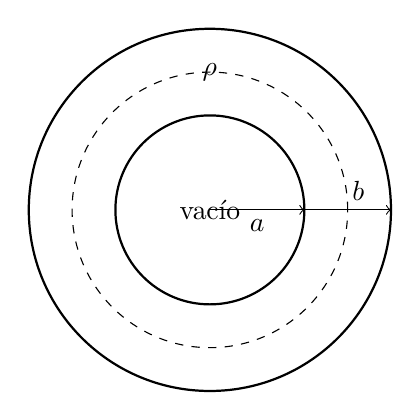
\begin{tikzpicture}[scale=1]

\draw[thick] (0,0) circle (1.2);
\draw[thick] (0,0) circle (2.3);

\draw[dashed] (0,0) circle (1.75);

\draw[->] (0,0) -- (1.2,0)
node[midway,below] {$a$};

\draw[->] (0,0) -- (2.3,0)
node[pos=0.82,above] {$b$};

\node at (0,0) {vacío};
\node at (0,1.75) {$\rho$};

\end{tikzpicture}
\end{center}

Determine el campo eléctrico en las tres regiones:

\[
r<a,\qquad
a<r<b,\qquad
r>b.
\]

\end{ejercicio}

\begin{respuesta}

\[
\boxed{E=0\qquad(r<a)}
\]

\[
\boxed{
E=
\frac{\rho(r^2-a^2)}{2\varepsilon_0r}
\qquad(a<r<b)
}
\]

\[
\boxed{
E=
\frac{\rho(b^2-a^2)}{2\varepsilon_0r}
\qquad(r>b)
}
\]

\end{respuesta}

\begin{explicacion}

Utilizamos una superficie gaussiana cilíndrica coaxial de radio \(r\) y longitud
\(L\).

Para

\[
r<a,
\]

la superficie no encierra carga:

\[
Q_{\text{enc}}=0.
\]

Entonces,

\[
E(2\pi rL)=0,
\]

por lo que

\[
\boxed{E=0}.
\]

Para

\[
a<r<b,
\]

la sección cargada encerrada es un anillo de área

\[
\pi(r^2-a^2).
\]

Por tanto,

\[
Q_{\text{enc}}
=
\rho\pi(r^2-a^2)L.
\]

Aplicamos Gauss:

\[
E(2\pi rL)
=
\frac{\rho\pi(r^2-a^2)L}{\varepsilon_0}.
\]

Despejando,

\[
\boxed{
E=
\frac{\rho(r^2-a^2)}{2\varepsilon_0r}
}.
\]

Para

\[
r>b,
\]

toda la distribución queda encerrada:

\[
Q_{\text{enc}}
=
\rho\pi(b^2-a^2)L.
\]

Entonces,

\[
E(2\pi rL)
=
\frac{\rho\pi(b^2-a^2)L}{\varepsilon_0}.
\]

Así,

\[
\boxed{
E=
\frac{\rho(b^2-a^2)}{2\varepsilon_0r}
}.
\]

\end{explicacion}


\begin{ejercicio}

Una distribución infinita de carga ocupa la región

\[
-a<x<a
\]

y posee densidad volumétrica uniforme positiva \(\rho\).

Determine la componente \(E_x\) del campo eléctrico:

\begin{enumerate}
    \item dentro de la distribución;
    \item fuera de ella.
\end{enumerate}

\end{ejercicio}

\begin{respuesta}

Para \(|x|<a\),

\[
\boxed{
E_x=\frac{\rho x}{\varepsilon_0}
}
\]

Para \(x>a\),

\[
\boxed{
E_x=+\frac{\rho a}{\varepsilon_0}
}
\]

Para \(x<-a\),

\[
\boxed{
E_x=-\frac{\rho a}{\varepsilon_0}
}
\]

\end{respuesta}

\begin{explicacion}

La distribución posee simetría respecto del plano \(x=0\).

Para un punto interior, elegimos una superficie gaussiana simétrica que se extienda
desde \(-x\) hasta \(+x\), con cada tapa de área \(A\).

El flujo atraviesa las dos tapas:

\[
\Phi_E=2EA.
\]

La carga encerrada es

\[
Q_{\text{enc}}
=
\rho(2xA).
\]

Aplicamos Gauss:

\[
2EA
=
\frac{2\rho xA}{\varepsilon_0}.
\]

Entonces,

\[
E=\frac{\rho|x|}{\varepsilon_0}.
\]

Considerando el sentido mediante la componente rectangular,

\[
\boxed{
E_x=\frac{\rho x}{\varepsilon_0}
\qquad(|x|<a)
}.
\]

Fuera de la distribución, toda la carga comprendida entre \(-a\) y \(+a\) queda
encerrada:

\[
Q_{\text{enc}}=2\rho aA.
\]

Por tanto,

\[
2EA
=
\frac{2\rho aA}{\varepsilon_0},
\]

de donde

\[
E=\frac{\rho a}{\varepsilon_0}.
\]

Para \(x>a\), el campo apunta hacia \(+x\):

\[
\boxed{
E_x=+\frac{\rho a}{\varepsilon_0}
}.
\]

Para \(x<-a\),

\[
\boxed{
E_x=-\frac{\rho a}{\varepsilon_0}
}.
\]

\end{explicacion}


\begin{ejercicio}

Dos láminas infinitas paralelas están situadas en

\[
x=-\frac d2
\qquad\text{y}\qquad
x=+\frac d2.
\]

La lámina izquierda posee densidad \(+\sigma\) y la derecha densidad \(-\sigma\).

Determine \(E_x\) en las tres regiones del espacio.

\begin{center}
\begin{tikzpicture}[>=Latex,scale=0.9]

\draw[very thick] (-2,-2) -- (-2,2);
\draw[very thick] (2,-2) -- (2,2);

\node[above] at (-2,2) {$+\sigma$};
\node[above] at (2,2) {$-\sigma$};

\draw[->] (-4,-2.6) -- (4,-2.6) node[right] {$x$};

\draw[<->] (-2,-2.2) -- (2,-2.2)
node[midway,above] {$d$};

\end{tikzpicture}
\end{center}

\end{ejercicio}

\begin{respuesta}

\[
\boxed{E_x=0\qquad x<-\frac d2}
\]

\[
\boxed{
E_x=\frac{\sigma}{\varepsilon_0}
\qquad
-\frac d2<x<\frac d2
}
\]

\[
\boxed{E_x=0\qquad x>\frac d2}
\]

\end{respuesta}

\begin{explicacion}

Cada lámina produce un campo de magnitud

\[
E_0=\frac{\sigma}{2\varepsilon_0}.
\]

A la izquierda de ambas láminas, el campo de \(+\sigma\) apunta hacia la izquierda,
mientras que el de \(-\sigma\) apunta hacia la derecha.

Por tanto,

\[
E_x=-E_0+E_0=0.
\]

Entre las láminas, ambos campos apuntan desde la lámina positiva hacia la negativa,
es decir, hacia \(+x\).

Entonces,

\[
E_x=E_0+E_0
=\frac{\sigma}{\varepsilon_0}.
\]

A la derecha de ambas láminas, las contribuciones vuelven a cancelarse:

\[
E_x=E_0-E_0=0.
\]

Por tanto,

\[
\boxed{
E_x=
\begin{cases}
0, & x<-\dfrac d2,\\[0.5em]
\dfrac{\sigma}{\varepsilon_0},
& -\dfrac d2<x<\dfrac d2,\\[0.8em]
0, & x>\dfrac d2.
\end{cases}
}
\]

\end{explicacion}


\begin{ejercicio}

Dos láminas infinitas paralelas poseen la misma densidad superficial positiva
\(+\sigma\) y están situadas en

\[
x=-\frac d2
\qquad\text{y}\qquad
x=+\frac d2.
\]

Determine \(E_x\) a la izquierda, entre las láminas y a la derecha.

\end{ejercicio}

\begin{respuesta}

\[
\boxed{
E_x=-\frac{\sigma}{\varepsilon_0}
\qquad x<-\frac d2
}
\]

\[
\boxed{
E_x=0
\qquad
-\frac d2<x<\frac d2
}
\]

\[
\boxed{
E_x=+\frac{\sigma}{\varepsilon_0}
\qquad x>\frac d2
}
\]

\end{respuesta}

\begin{explicacion}

Cada lámina positiva produce un campo que apunta alejándose de ella y tiene magnitud

\[
E_0=\frac{\sigma}{2\varepsilon_0}.
\]

A la izquierda de ambas, los dos campos apuntan hacia \(-x\):

\[
E_x=-E_0-E_0
=-\frac{\sigma}{\varepsilon_0}.
\]

Entre las láminas, una contribución apunta hacia \(+x\) y la otra hacia \(-x\):

\[
E_x=E_0-E_0=0.
\]

A la derecha de ambas, las dos contribuciones apuntan hacia \(+x\):

\[
E_x=E_0+E_0
=+\frac{\sigma}{\varepsilon_0}.
\]

Por tanto,

\[
\boxed{
E_x=
\begin{cases}
-\dfrac{\sigma}{\varepsilon_0},
& x<-\dfrac d2,\\[0.8em]
0,
& -\dfrac d2<x<\dfrac d2,\\[0.8em]
+\dfrac{\sigma}{\varepsilon_0},
& x>\dfrac d2.
\end{cases}
}
\]

\end{explicacion}


\begin{ejercicio}

Una carga puntual positiva \(q\) se encuentra en el centro de una esfera imaginaria
de radio \(R\).

Considere solamente la mitad superior de la superficie esférica, sin incluir el
disco de su base.

Determine el flujo eléctrico a través de esta superficie hemisférica.

\end{ejercicio}

\begin{respuesta}

\[
\boxed{
\Phi_E=\frac{q}{2\varepsilon_0}
}
\]

\end{respuesta}

\begin{explicacion}

El flujo total a través de una esfera completa centrada en la carga es

\[
\Phi_{\text{esfera}}
=
\frac{q}{\varepsilon_0}.
\]

La distribución del campo sobre la esfera es completamente simétrica.

Por tanto, cada hemisferio recibe exactamente la mitad del flujo:

\[
\Phi_{\text{hemisferio}}
=
\frac12\Phi_{\text{esfera}}.
\]

Así,

\[
\boxed{
\Phi_E=\frac{q}{2\varepsilon_0}
}.
\]

También puede obtenerse directamente utilizando

\[
E=k\frac{q}{R^2}
\]

y el área curva del hemisferio,

\[
A=2\pi R^2.
\]

Como el campo es perpendicular a la superficie curva,

\[
\Phi_E=EA
=
k\frac{q}{R^2}(2\pi R^2)
=
2\pi kq
=
\frac{q}{2\varepsilon_0}.
\]

\end{explicacion}


\begin{ejercicio}

Una carga puntual \(q\) se encuentra dentro de una superficie gaussiana esférica,
pero no está situada en su centro.

Determine el flujo eléctrico neto a través de la esfera.

¿Puede calcularse el campo eléctrico sobre toda la superficie mediante

\[
E(4\pi R^2)=\frac{q}{\varepsilon_0}?
\]

Explique.

\end{ejercicio}

\begin{respuesta}

\[
\boxed{
\Phi_E=\frac{q}{\varepsilon_0}
}
\]

No puede utilizarse

\[
E(4\pi R^2)=\frac{q}{\varepsilon_0}
\]

para obtener un único valor de \(E\) sobre la esfera.

\end{respuesta}

\begin{explicacion}

La ley de Gauss depende únicamente de la carga neta encerrada.

Como la esfera encierra \(q\),

\[
\boxed{
\Phi_E=\frac{q}{\varepsilon_0}
}.
\]

Sin embargo, al estar la carga fuera del centro, la distancia entre la carga y los
distintos puntos de la esfera no es constante.

Por ello, la magnitud del campo tampoco es constante sobre la superficie.

Además, el campo no es necesariamente perpendicular a la esfera en todos los puntos.

En consecuencia, no puede escribirse

\[
\oint E\cos\theta\,dA
=
E\oint dA.
\]

La ley de Gauss continúa siendo válida, pero la simetría no permite despejar \(E\)
mediante

\[
E(4\pi R^2).
\]

\end{explicacion}


\begin{ejercicio}

En el interior de una distribución de carga con simetría esférica se encuentra
experimentalmente que el campo eléctrico tiene magnitud

\[
E(r)=Cr,
\]

donde \(C>0\) es constante y el campo apunta radialmente hacia afuera.

Determine la densidad volumétrica de carga \(\rho\).

\end{ejercicio}

\begin{respuesta}

\[
\boxed{\rho=3\varepsilon_0C}
\]

\end{respuesta}

\begin{explicacion}

Tomamos una superficie gaussiana esférica de radio \(r\).

Por simetría,

\[
\Phi_E=E(4\pi r^2).
\]

Como

\[
E=Cr,
\]

entonces

\[
\Phi_E=(Cr)(4\pi r^2)
=4\pi Cr^3.
\]

Por la ley de Gauss,

\[
Q_{\text{enc}}
=
\varepsilon_0\Phi_E.
\]

Así,

\[
Q_{\text{enc}}
=
4\pi\varepsilon_0Cr^3.
\]

Para una densidad volumétrica uniforme,

\[
Q_{\text{enc}}
=
\rho\frac43\pi r^3.
\]

Igualando,

\[
\rho\frac43\pi r^3
=
4\pi\varepsilon_0Cr^3.
\]

Cancelamos \(4\pi r^3\):

\[
\frac{\rho}{3}
=
\varepsilon_0C.
\]

Por tanto,

\[
\boxed{\rho=3\varepsilon_0C}.
\]

El hecho de que \(E\propto r\) es consistente con una densidad volumétrica uniforme.

\end{explicacion}


\begin{ejercicio}

Una esfera aislante de radio \(R\) posee una densidad volumétrica con simetría
esférica dada por

\[
\rho(r)=\rho_0\left(1-\frac{r}{R}\right),
\qquad 0\leq r\leq R,
\]

donde \(\rho_0>0\).

Determine:

\begin{enumerate}
    \item el campo eléctrico para \(r<R\);
    \item la carga total de la esfera;
    \item el campo eléctrico para \(r>R\).
\end{enumerate}

\end{ejercicio}

\begin{respuesta}

Para \(r<R\),

\[
\boxed{
E(r)
=
\frac{\rho_0}{\varepsilon_0}
\left(
\frac{r}{3}
-
\frac{r^2}{4R}
\right)
}
\]

La carga total es

\[
\boxed{
Q=\frac{\pi\rho_0R^3}{3}
}
\]

Para \(r>R\),

\[
\boxed{
E(r)
=
\frac{\rho_0R^3}
{12\varepsilon_0r^2}
}
\]

\end{respuesta}

\begin{explicacion}

Para \(r<R\), la carga encerrada debe calcularse integrando:

\[
Q_{\text{enc}}
=
\int_0^r\rho(r')\,4\pi r'^2\,dr'.
\]

Sustituimos

\[
\rho(r')
=
\rho_0\left(1-\frac{r'}{R}\right).
\]

Entonces,

\[
Q_{\text{enc}}
=
4\pi\rho_0
\int_0^r
\left(
r'^2-\frac{r'^3}{R}
\right)dr'.
\]

Integrando,

\[
Q_{\text{enc}}
=
4\pi\rho_0
\left(
\frac{r^3}{3}
-
\frac{r^4}{4R}
\right).
\]

Aplicamos la ley de Gauss:

\[
E(4\pi r^2)
=
\frac{Q_{\text{enc}}}{\varepsilon_0}.
\]

Por tanto,

\[
E
=
\frac{\rho_0}{\varepsilon_0}
\left(
\frac{r}{3}
-
\frac{r^2}{4R}
\right).
\]

Así,

\[
\boxed{
E(r)
=
\frac{\rho_0}{\varepsilon_0}
\left(
\frac{r}{3}
-
\frac{r^2}{4R}
\right)
\qquad(r<R)
}.
\]

Para obtener la carga total, hacemos \(r=R\):

\[
Q
=
4\pi\rho_0
\left(
\frac{R^3}{3}
-
\frac{R^3}{4}
\right).
\]

Como

\[
\frac13-\frac14=\frac1{12},
\]

resulta

\[
Q
=
4\pi\rho_0R^3\left(\frac1{12}\right)
=
\boxed{\frac{\pi\rho_0R^3}{3}}.
\]

Para \(r>R\), toda la carga queda encerrada:

\[
E(4\pi r^2)
=
\frac{Q}{\varepsilon_0}.
\]

Sustituyendo el valor de \(Q\),

\[
E
=
\frac{1}{4\pi\varepsilon_0r^2}
\frac{\pi\rho_0R^3}{3}.
\]

Simplificando,

\[
\boxed{
E(r)
=
\frac{\rho_0R^3}
{12\varepsilon_0r^2}
\qquad(r>R)
}.
\]

\end{explicacion}